\chapter{Schermate dell'applicazione}

\counterwithout{figure}{chapter}
\counterwithout{table}{chapter}
\counterwithin{figure}{chapter}
\counterwithin{table}{chapter}

\begin{figure}[h!]
    \centering    
        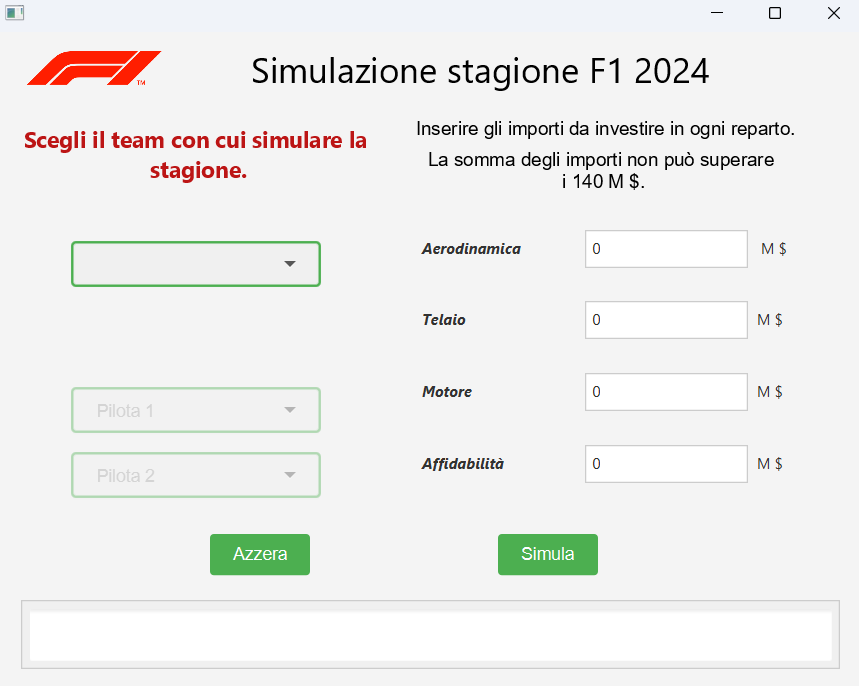
\includegraphics[width=\textwidth]{Figures/schermata1.png}
        \caption{Schermata di simulazione vuota}
        \label{fig:schermata_simulazione_vuota}
\end{figure}
\begin{figure}[h!]
        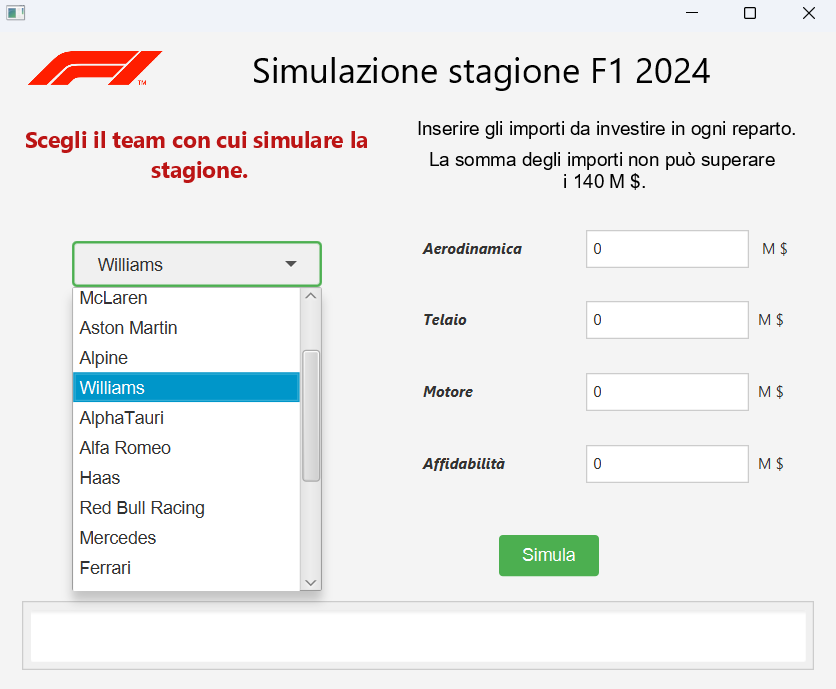
\includegraphics[width=\textwidth]{Figures/schermata2.png}
        \caption{Selezionamento della scuderia tramite la ComboBox}
        \label{fig:selezionamento_scuderia}
\end{figure}

\begin{figure}[h!]
    \centering
    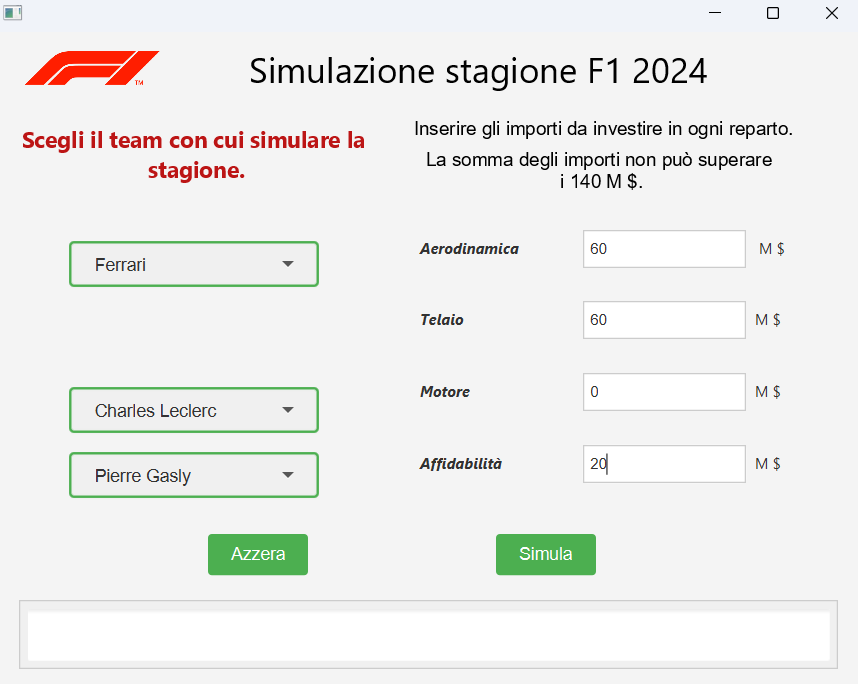
\includegraphics[width=\textwidth]{Figures/schermata3.png}
    \caption{Schermata di simulazione con i parametri impostati correttamente}
    \label{fig:schermata_simulazione_parametri}
\end{figure}

\begin{figure}[h!]
    \centering
        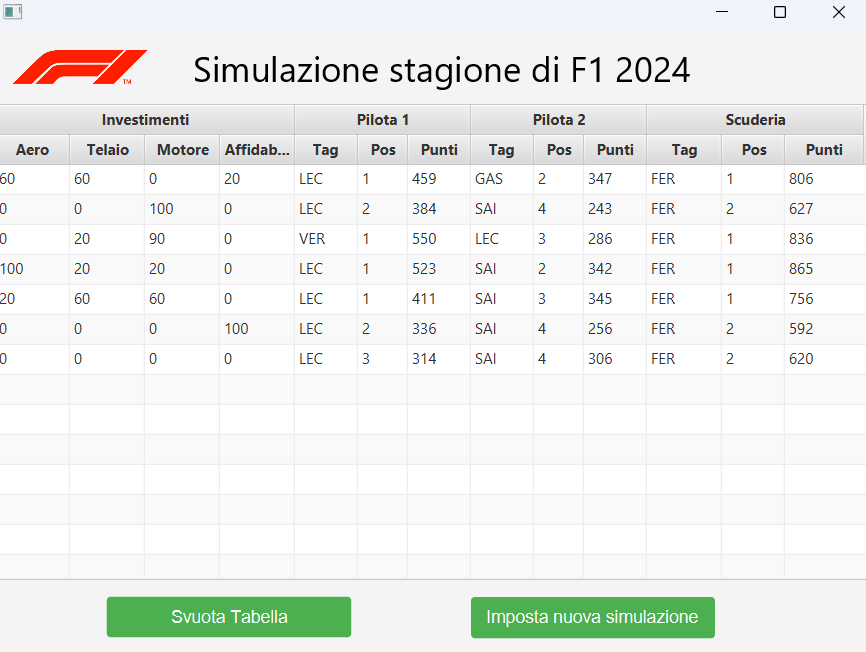
\includegraphics[width=\textwidth]{Figures/schermata4.png}
        \caption{Tabella riepilogativa con i risultati delle simulazioni svolte con un solo team}
        \label{fig:tabella_riepilogativa_singolo_team}
    \hspace{1cm}
        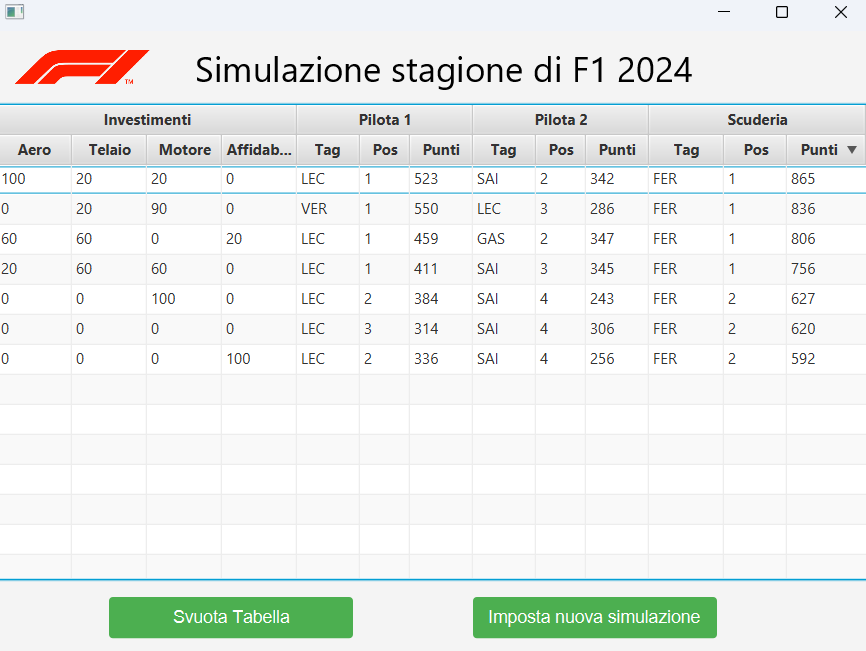
\includegraphics[width=\textwidth]{Figures/ordinata.png}
        \caption{Tabella riepilogativa ordinata in base al punteggio finale nella classifica costruttori}
        \label{fig:tabella_riepilogativa_ordine_punteggio}
\end{figure}

\begin{figure}[h!]
    \centering
    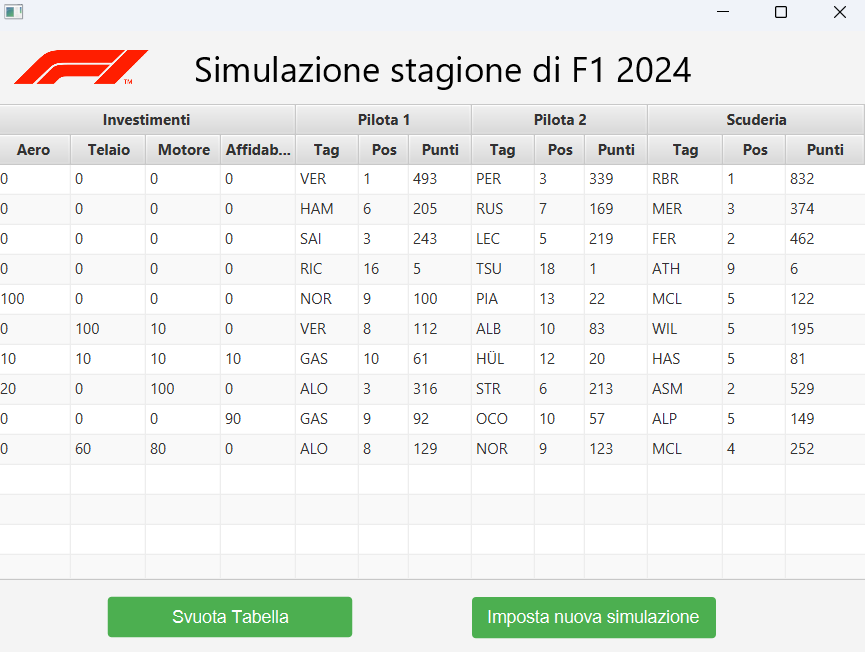
\includegraphics[width=\textwidth]{Figures/schermata5.png}
    \caption{Tabella riepilogativa con i risultati delle simulazioni svolte con diversi team}
    \label{fig:tabella_riepilogativa_diversi_team}


\vspace{8cm}
È disponibile un video sulla piattaforma di YouTube che spiega e dimostra il funzionamento dell'applicazione.

\hypersetup{
    colorlinks=true,
    linkcolor=blue,
    urlcolor=blue
}

Link al video: \href{https://youtu.be/1NBmYkZLF8o?si=xOuhJ_83H7A89qkq}{\texttt{https://youtu.be/1NBmYkZLF8o?si=xOuhJ_83H7A89qkq}}.

\end{figure}
